\section{Αριθμός πλεγματικών θέσεων που το σωματίδιο επισκέφτηκε τουλάχιστον μία φορά}
\subsection{Σε μία διάσταση}
\label{S1D}
Η λογική που θα εκτελεστεί το πείραμα είναι προφανώς παρόμοια με τα προηγούμενα πειράματα μιας και πρόκειται για μονοδιάστατο τυχαίο περίπατο. Πάμε πρώτα να μελετήσουμε πως θα εκτελεστεί το ένα πείραμα σε αυτή την περίπτωση και έπειτα στον τελικό κώδικα θα τρέξει για {\en runs}=10000 φορές. 

Ψάχνουμε να υπολογίσουμε τον αριθμό των διαφορετικών θέσεων που έχει λάβει το σωματίδιο κατά το ταξίδι του στην γραμμή των ακεραίων αριθμών $\mathbb{Z}$. Θα εκμεταλλευτούμε το γεγονός ότι στη μία διάσταση ο μόνος τρόπος να μεταβεί το σωματίδιο στη θέση $n>0$ είναι πρώτα να έχει περάσει από τις θέσεις $n-1,n-2...1$, μιας και η εκκίνηση πάντα γίνεται από το $0$. Ομοίως, για να έχει βρεθεί στην θέση $-n<0$ θα πρέπει να έχει περάσει από τις $-n+1,-n+2...$ κ.ο.κ. Επομένως, αν γνωρίζουμε τις δύο μεγαλύτερες αποστάσεις (μία προς τα θετικά μία προς τα αρνητικά) από το σημείο εκκίνησης, είμαστε σίγουροι ότι το σωματίδιο έχει περάσει από όλες τις ενδιάμεσες τοποθεσίες. Έτσι, μπορούμε να βρούμε την {\en maximum} και την {\en minimum} θέση, και να υπολογίσουμε τον αριθμό των διαφορετικών θέσεων με την φόρμουλα $maxpos-minpos+1$. Από την μέγιστη θέση αφαιρούμε την αρνητική ελάχιστη θέση, και προσθέτουμε 1 (για να συμπεριληφθεί και η αρχική θέση 0). Για παράδειγμα, αν η μέγιστη θέση είναι 5 και η ελάχιστη -2, τότε ο αριθμός των διαφορετικών θέσεων θα είναι 5-(-2)+1=8 όπου αναφέρεται στις θέσεις -2,-1,0,1,2,3,4,5.
Όπως και πριν, πρέπει να κρατήσουμε τους αριθμούς των 10000 πειραμάτων ανά 100 βήματα επομένως πάλι θα πρέπει να αρχικοποιήσουμε μία 10-λίστα {\en \texttt{s\_t}} με μηδενικά. Σε αυτή θα προσθέτουμε κάθε 100 βήματα (από 100 μέχρι 1000) τον αριθμό $S$ των διαφορετικών θέσεων. 
Ο αλγόριθμος ενός πειράματος: 
\en
\begin{lstlisting}
//=============================================================//
set starting position
set min and max variables to zero
for 1000 steps:
    update position randomly(left or right)
    if position bigger than max set position as max
    if position smaller than min set position as min
    if step 100 or 200 or......1000:
           add to s_t list
//=============================================================//
\end{lstlisting}
\gr
ο κώδικας που τον υλοποιεί:
\en
\begin{python}
position = 0
min_pos = 0
max_pos = 0
for t in range(1,1001):
    move = random.choice([-step,+step])
    position+= move
    if position<min_pos:
        min_pos = position
    elif position>max_pos:
        max_pos = position
    if t%100==0:
        s_t[t//100-1]+= max_pos-min_pos+1
\end{python}
\gr 
Παρατηρείστε ότι η εντολή {\en \texttt{s\_t[t//100-1]+= max\_pos-min\_pos+1}} προσθέτει στην θέση 0 της λίστας, τον αριθμό των διαφορετικών θέσεων που επισκέφτηκε το σωματίδιο στα 100 βήματα, στην θέση 1 της λίστας των 200 βημάτων κ.ο.κ.
\newpage
\noindent
Ο συνολικός κώδικας:
\en
\begin{python}
start_time = time.time()

runs = 10000
step = 1
s_t = [0]*10
for i in range(runs):
    position = 0
    min_pos = 0
    max_pos = 0
    for t in range(1,1001):
        move = random.choice([-step,+step])
        position+= move
        if position<min_pos:
            min_pos = position
        elif position>max_pos:
            max_pos = position
        if t%100==0:
            s_t[t//100-1]+= max_pos-min_pos+1
mean_s = np.array([(x/runs) for x in s_t])

print(f"Average Number of Distinct Sites per 100 steps:{mean_s}")
print(f"Execution Time: {(time.time() - start_time)} seconds.")
\end{python}
\gr όπου απευθείας δημιουργούμε την {\en numpy array} με τις μέσες τιμές των διαφορετικών θέσεων ανά 100 βηματισμούς για όλα τα 10000 {\en runs}.
To {\en output}:
\en
\begin{python}
Average Number of Distinct Sites per 100 steps:[15.9749 
                                                22.5574 
                                                27.4858 
                                                31.6908 
                                                35.4432 
                                                38.8125 
                                                41.9199 
                                                44.8198 
                                                47.5799
                                                50.197 ]
Execution Time: 7.148834943771362 seconds.
\end{python}
\gr 
Κατασκευάζουμε τώρα το γράφημα με τετμημένη των αριθμό των βημάτων όπου δημιουργούμε με την εντολή {\en np.arange} και τεταγμένη τους μέσους αριθμούς {\en \texttt{mean\_s}}. 
\newpage
\noindent
Ο κώδικας: 
\en 
\begin{python}
t = np.arange(100,1001,100)
plt.plot(t, mean_s, '.-',color = 'red', ms = 10)
plt.grid(color='0.25', linestyle='--', linewidth=0.2)
plt.ylabel('Number of Distinct Sites Visited')
plt.xlabel('Number of Random Steps')
plt.title('Discrete Random Walk - Number of Distinct Sites-1D')
plt.show()
\end{python}
\gr με {\en output}:
\begin{figure}[H]
\begin{center}
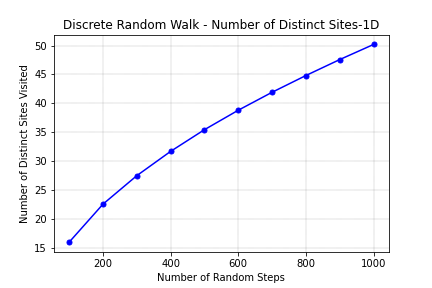
\includegraphics[scale=1]{figures/DRW_NDS_1D.png}
\caption{Μέσος αριθμός διαφορετικών τοποθεσιών σε μία διάσταση, που το σωματίδιο επισκέφτηκε τουλάχιστον μία φορά.}
\label{figuridion3d}
\end{center}
\end{figure}

\subsection{Σε δύο διαστάσεις}
\label{S2D}
Στην περίπτωση των δύο διαστάσεων η λογική παραμένει η ίδια όμως χρειάζονται τροποποιήσεις. Η πρώτη τροποποίηση αφορά την επιλογή της επόμενης κίνησης όπως έγινε και σε προηγούμενο πείραμα. Επιλέγουμε τυχαία και ομοιόμορφα μία από τις κινήσεις πάνω, κάτω, αριστερά, δεξιά και ανανεώνουμε την θέση του σωματιδίου. 
Η δεύτερη τροποποίηση έχει να κάνει με την γνώση μας για το αν η θέση που θα μεταβαίνει το σωματίδιο είναι μία από τις θέσεις που έχει επισκεφθεί προηγουμένως. Το τρικ που χρησιμοποιήσαμε στην περίπτωση της μίας διάστασης δεν δουλεύει στην περίπτωση των δύο διαστάσεων. Το γεγονός ότι το σωματίδιο βρίσκεται στην θέση $(x,y)$ μας εξασφαλίζει ότι έχει βρεθεί σε μία εκ των $(x-1,y),(x+1,y),(x,y-1),(x,y+1)$ χωρίς όμως να γνωρίζουμε ποια 'η ποιες. Ως αποτέλεσμα αυτού, πρέπει σε κάθε βήμα να ελέγχουμε αν η ανανεωμένη θέση είναι θέση που έχει επισκεφτεί το σωματίδιο προηγουμένως. Γι' αυτό και σε κάθε πείραμα θα πρέπει να αποθηκεύουμε όλες τις νέες θέσεις που επισκέπτεται το σωματίδιο σε μία λίστα ονόματι {\en \texttt{all\_positions}}. Στο τέλος το μήκος αυτής της λίστας θα είναι και ο αριθμός των διαφορετικών θέσεων που έχει επισκεφθεί το σωματίδιο. Φυσικά διατηρούμε τη στρατηγική των ανά 100 μέσων όρων για τα 10000 {\en runs} με χρήση της λίστας \texttt{s\_t}. Ο αλγόριθμός του ενός πειράματος έχει ως εξής:
\en
\begin{lstlisting}
//=============================================================//
set starting position
set list of different positions visited
for 1000 steps:
    update position randomly(left, right, up, down)
    if position not visited before:
           add new position to the list of different positions
    if steps 100 or 200 ....:
           add length of the different pos list to the s_t list           
//=============================================================//
\end{lstlisting}
\gr 
Ο κώδικας που υλοποιεί το ένα πείραμα: 
\en
\begin{python}
position_x = 0
position_y = 0 
all_positions = [[0,0]]
for j in range(1,t+1):
    move = random.choice([[-step,0],[step,0],[0,-step],[0,step]])
    position_x+= move[0]
    position_y+= move[1]
    position = [position_x,position_y]
    if position not in all_positions:
        all_positions.append(position)
    if j%100==0:
        s_t[j//100-1]+= len(all_positions)
\end{python}
\gr Προφανώς όπως και πριν, η {\en \texttt{s\_t}} αρχικοποιείται με μηδενικά στο τελικό πρόγραμμα ώστε να λειτουργήσει για όλα τα {\en runs}. Ας σημειώσουμε εδώ ότι η λίστα {\en \texttt{all\_positions}} έχει ως μέλη της, λίστες μήκους 2, που αναπαριστούν την τετμημένη και την τεταγμένη των διαφορετικών θέσεων. 
\newpage
\noindent
Ο συνολικός κώδικας:
\en 
\begin{python}
start_time = time.time()

runs = 10000
step = 1
s_t = [0]*10
t = 1000
for i in range(runs):
    position_x = 0
    position_y = 0 
    all_positions = [[0,0]]
    for j in range(1,t+1):
        move = random.choice([[-step,0],[step,0],[0,-step],[0,step]])
        position_x+= move[0]
        position_y+= move[1]
        position = [position_x,position_y]
        if position not in all_positions:
            all_positions.append(position)
        if j%100==0:
            s_t[j//100-1]+= len(all_positions)

mean_s = np.array([(x/runs) for x in s_t])

print(f"Average Number of Distinct Sites per 100 steps:{mean_s}")
print(f"Execution Time: {(time.time() - start_time)} seconds.")
\end{python}
\gr 
με έξοδο
\en
\begin{python}
Average Number of Distinct Sites per 100 steps:[49.4849
                                                89.0422 
                                                126.3679 
                                                162.2419 
                                                197.2506 
                                                231.6082 
                                                265.2785 
                                                298.4961
                                                331.2296 
                                                363.4049]
Execution Time: 40.61035513877869 seconds.
\end{python}
\gr 
\newpage
\noindent
Κατασκευάζουμε όμοια με πριν το γράφημα:
\en
\begin{python}
t = np.arange(100,1001,100)
plt.plot(t, mean_s, '.-',color = 'blue', ms = 10)
plt.grid(color='0.25', linestyle='--', linewidth=0.2)
plt.ylabel('Number of Distinct Sites Visited')
plt.xlabel('Number of Random Steps')
plt.title('Discrete Random Walk - Number of Distinct Sites-2D')
plt.savefig('../pdf/figures/DRW_NDS_2D.png')
plt.show()
\end{python}
\gr 
\begin{figure}[H]
\begin{center}
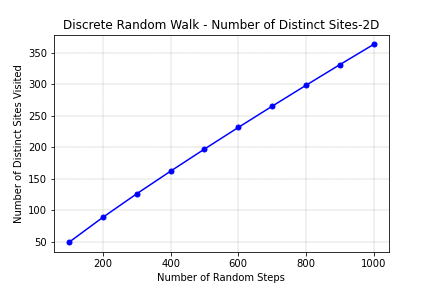
\includegraphics[scale=1]{figures/DRW_NDS_2D.png}
\caption{Μέσος αριθμός διαφορετικών τοποθεσιών σε δύο διαστάσεις, που το σωματίδιο επισκέφτηκε τουλάχιστον μία φορά.}
\label{figuridion3d}
\end{center}
\end{figure}